\apendice{Plan de Proyecto Software}




\section{Introducción}

Este Trabajo Fin de Grado se ha gestionado con \textbf{Scrum}, un marco de trabajo ágil orientado a la entrega iterativa e incremental de valor. Scrum se basa en el \emph{control empírico de procesos} (transparencia, inspección y adaptación) y estructura el desarrollo en iteraciones cortas llamadas \emph{sprints}, con artefactos y eventos bien definidos que favorecen el enfoque, la priorización y la mejora continua.

\subsection*{Scrum}
\textbf{Roles.} En este proyecto los roles se han adaptado de forma pragmática:
\begin{itemize}
	\item \textbf{Product Owner (PO):} el propio estudiante, responsable de priorizar el \emph{Product Backlog} alineado con los objetivos del TFG y las indicaciones de los tutores.
	\item \textbf{Scrum Master (SM):} rol asumido también por el estudiante, velando por la correcta aplicación del marco y la eliminación de impedimentos.
	\item \textbf{Equipo de desarrollo:} el estudiante (desarrollo, pruebas y documentación). \emph{Stakeholders}: tutores y tribunal.
\end{itemize}

\textbf{Artefactos.}
\begin{itemize}
	\item \textbf{Product Backlog:} lista priorizada de épicas e historias (documentación, investigación de modelos de IA de procesado de imágenes, pruebas comparativas, etc.).
	\item \textbf{Sprint Backlog:} subconjunto comprometido para cada sprint, desglosado en tareas técnicas.
	\item \textbf{Incremento:} entregables verificables al final de cada sprint (p.\,ej., secciones de la memoria, scripts de prueba, comparativas).
\end{itemize}

\textbf{Eventos.}
\begin{itemize}
	\item \textbf{Sprint Planning:} definición del objetivo del sprint y selección de trabajo.
	\item \textbf{Daily Scrum:} chequeo diario (\emph{qué hice/haré/impedimentos}) para mantener foco.
	\item \textbf{Sprint Review:} revisión de avances con evidencias (código, resultados, documentación).
	\item \textbf{Sprint Retrospective:} lecciones aprendidas y acciones de mejora para el siguiente sprint.
\end{itemize}


\subsection*{Medición y estimación del trabajo}

Para la planificación y seguimiento del progreso se ha empleado un sistema de medición basado en puntos de historia, una unidad habitual en metodologías ágiles como Scrum.  
Cada tarea o ítem del \emph{Sprint Backlog} se ha valorado con un número de puntos que refleja su esfuerzo y complejidad relativa.  

En este proyecto, se ha establecido una equivalencia práctica de 8 puntos por jornada completa de trabajo, lo que permite estimar la carga de trabajo de cada sprint y evaluar el avance real frente al planificado.  
Este sistema facilita mantener una visión objetiva del esfuerzo invertido y ajustar la planificación de los siguientes sprints en función de la velocidad media alcanzada.



\section{Planificación temporal}

La planificación se organiza en sprints cortos (1–2 semanas).

\subsection*{Visión general del Sprint 1}
\begin{itemize}
	\item \textbf{Fechas:} 27/10 – 06/11
	\item \textbf{Objetivo del sprint:} \emph{Investigación y pruebas iniciales de IAs de procesado de imágenes}.
	\item \textbf{Criterio de aceptación global:} disponer de dos IAs instaladas y probadas con evidencias, y una comparativa preliminar documentada.
\end{itemize}

Tal y como se muestra en la Tabla~\ref{tabla:sprint1} y en la Figura~\ref{fig:sprint1}, este sprint se centra en la fase inicial de investigación y preparación del proyecto.

\begin{table}[h!]
	\centering
	
	\begin{tabular}{@{}llcll@{}}
		\toprule
		\textbf{Tarea} & \textbf{Pts} \\
		\midrule
		Organización inicial del proyecto & 8  \\
		Aprendizaje básico de \LaTeX      & 8   \\
		Estructura base del documento TFG & 8   \\
		Investigar modelos IA de imágenes & 8  \\
		Instalar y probar 1\textsuperscript{a} IA & 8  \\
		Instalar y probar 2\textsuperscript{a} IA & 8  \\
		Comparativa entre IAs seleccionadas & 8 &  \\
		Cierre Sprint                      & 8 &  \\
		\midrule
		\bottomrule
	\end{tabular}
	\caption{Sprint 1 – Resumen}
	\label{tabla:sprint1}
\end{table}

\begin{figure}[h!]
	\centering
	
	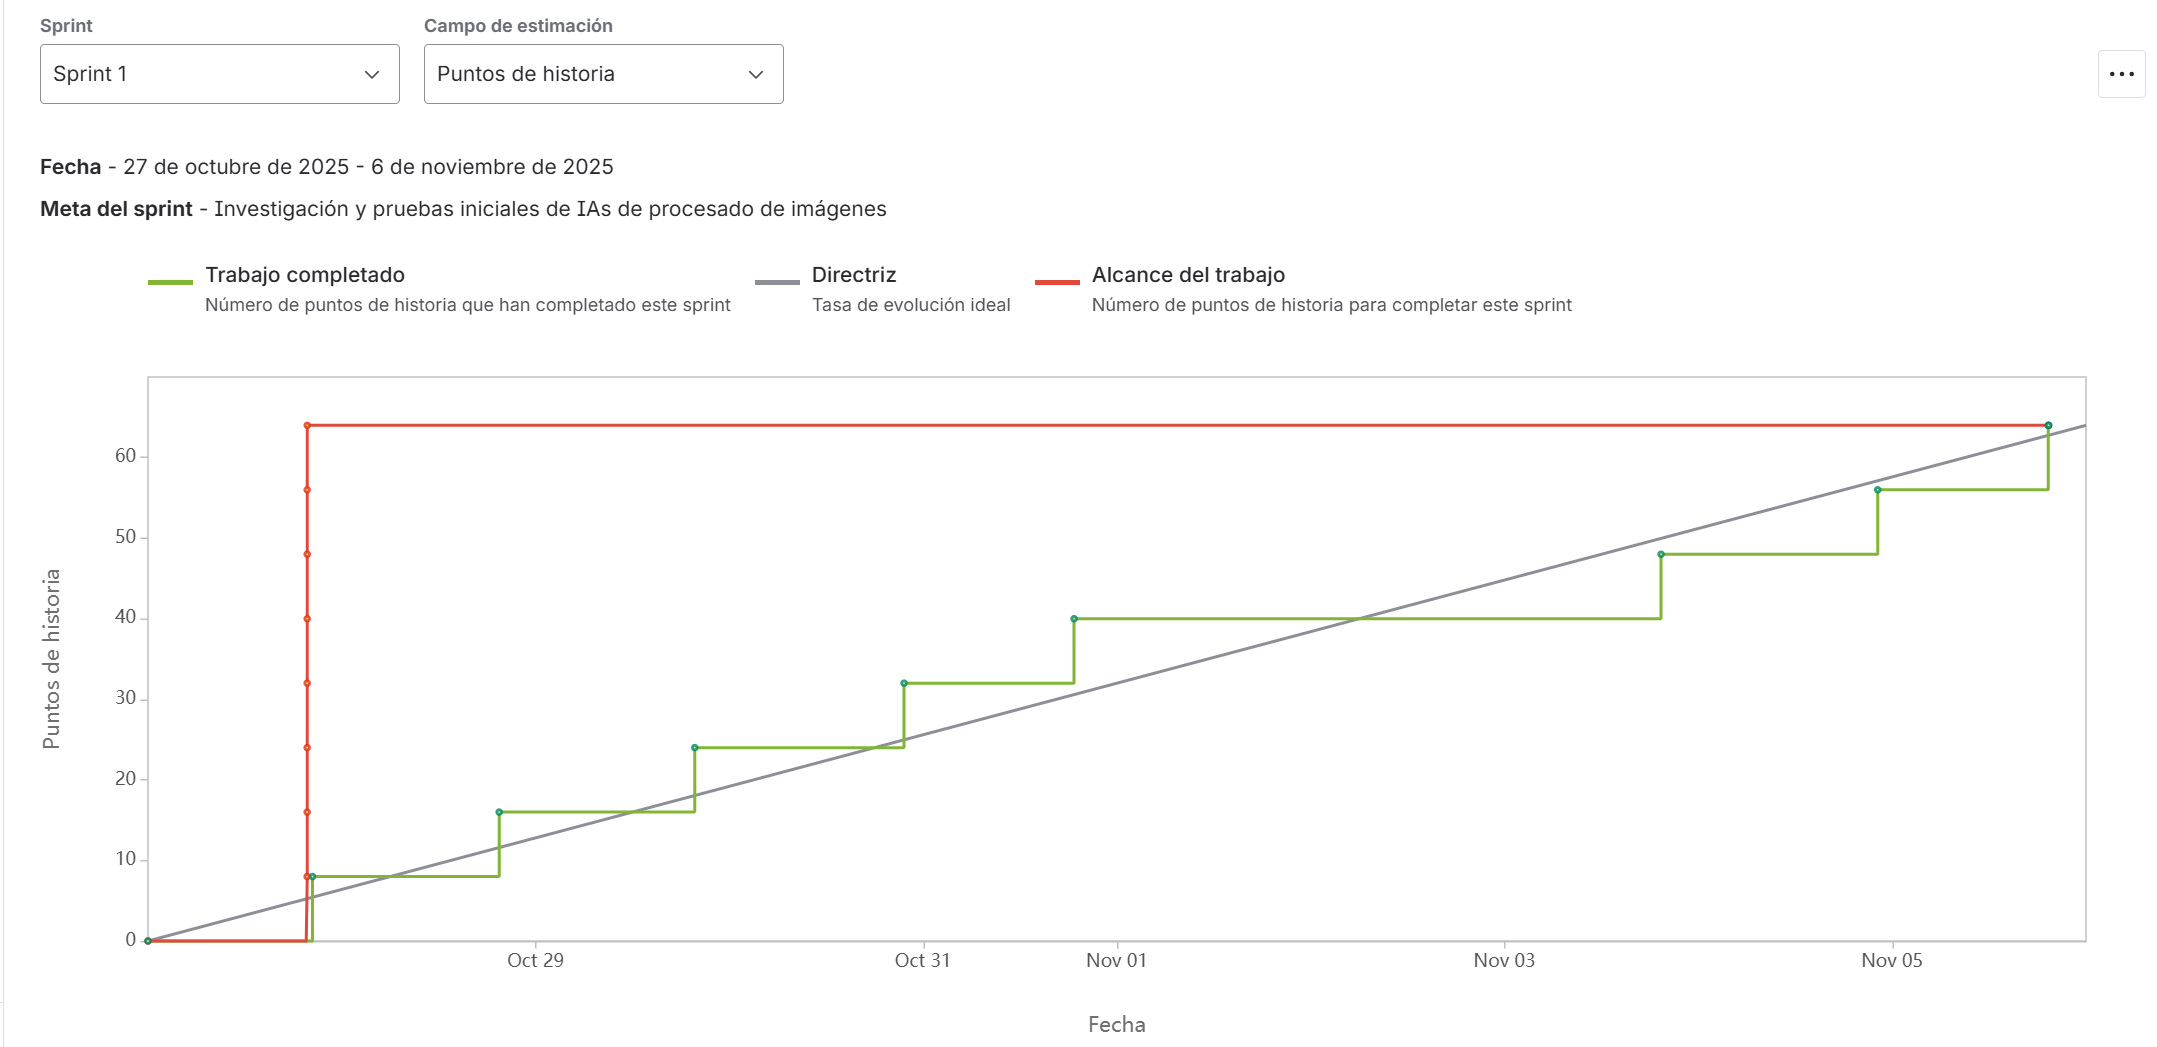
\includegraphics[width=0.95\textwidth]{img/sprint1.png}
	\caption{Informe de trabajo completado Sprint 1}
	\label{fig:sprint1}
\end{figure}


\subsubsection*{Descripción de las tareas del Sprint 1}

A continuación se describen brevemente las tareas que componen el Sprint 1:

\begin{itemize}
	\item \textbf{Organización inicial del proyecto.}  
	Se configuró el entorno de trabajo creando la estructura del repositorio, las carpetas para código, experimentos, documentación y resultados, así como los archivos necesarios para el control de versiones y la vinculación con Jira. Esta tarea permitió establecer la base técnica sobre la que se desarrollará el resto del proyecto.
	
	\item \textbf{Aprendizaje básico de \LaTeX.}  
	Se dedicó tiempo a adquirir soltura con la herramienta de edición científica \LaTeX, aprendiendo a crear capítulos, incluir figuras, tablas, referencias y bibliografía. Este conocimiento asegura una correcta elaboración y mantenimiento de la memoria del TFG.
	
	\item \textbf{Estructura base del documento TFG.}  
	Se definió la organización general de la memoria, creando los capítulos principales, anexos y secciones iniciales. De este modo quedó preparada la estructura en la que se irá incorporando el contenido teórico y técnico conforme avance el proyecto.
	
	\item \textbf{Investigar modelos IA de procesamiento de imágenes.}  
	Se llevó a cabo una investigación de diferentes alternativas de inteligencia artificial aplicadas al procesamiento de imágenes, evaluando su documentación, facilidad de uso, licencia y compatibilidad. Tras este estudio se seleccionaron dos herramientas destacadas: \textbf{YOLO} y \textbf{MediaPipe}, por su relevancia en el ámbito de la visión por computador.
	
	\item \textbf{Instalar y probar la primera IA seleccionada (YOLO).}  
	En esta tarea se instaló y configuró el modelo YOLO (You Only Look Once), mediante la librería \texttt{ultralytics} en Python. Se realizaron pruebas de detección de objetos sobre imágenes propias para verificar la correcta ejecución del modelo, su velocidad de inferencia y la claridad de sus resultados. Esta fase permitió comprobar la idoneidad de YOLO para el reconocimiento y localización de elementos dentro de una escena.
	
	\item \textbf{Instalar y probar la segunda IA seleccionada (MediaPipe).}  
	Posteriormente se instaló el framework MediaPipe de Google, que ofrece soluciones preentrenadas orientadas al análisis de características humanas como el rostro, las manos o la pose corporal. Se probaron distintos módulos, especialmente los de detección de manos y pose, verificando su funcionamiento en tiempo real y su facilidad de integración en proyectos Python.  
	
	\item \textbf{Comparativa entre las IAs seleccionadas.}  
	Una vez probadas ambas herramientas, se elaboró una comparativa que analiza sus principales diferencias: finalidad, precisión, velocidad, facilidad de uso, requerimientos y tipo de tareas para las que son más adecuadas.  
	En esta comparativa se concluye que \textbf{MediaPipe} destaca en la detección y seguimiento de características humanas con bajo coste computacional, mientras que \textbf{YOLO} ofrece mayor versatilidad para la detección general de objetos y escenarios más complejos. La documentación y análisis detallados de esta comparativa se incluyen en el capítulo 4 de la memoria.
	
	\item \textbf{Cierre del Sprint.}  
	Finalmente, se revisaron todas las tareas completadas y se documentaron los avances obtenidos, preparando el tablero y el backlog para el siguiente sprint. Esta revisión permitió valorar el cumplimiento de los objetivos y establecer las líneas de trabajo futuras.
\end{itemize}

\subsection*{Visión general del Sprint 2}
\begin{itemize}
	\item \textbf{Fechas:} 09/11 – 20/11
	\item \textbf{Objetivo del sprint:} \emph{Construir un servidor funcional en Flask capaz de recibir imágenes, ejecutar detecciones simuladas y ofrecer una interfaz mínima de usuario.}
	\item \textbf{Criterio de aceptación global:} disponer de un servidor operativo, con endpoints funcionales, selección de modelos simulada y una UI básica que permita validar el flujo completo de subida y procesado.
\end{itemize}

Tal y como se recoge en la Tabla~\ref{tabla:sprint2} y en la Figura~\ref{fig:sprint2}, este sprint introduce la construcción del servidor y la primera interfaz funcional.

\begin{table}[h!]
	\centering
	\begin{tabular}{@{}ll@{}}
		\toprule
		\textbf{Tarea} & \textbf{Pts} \\
		\midrule
		Definir alcance del sprint y crear historias & 8 \\
		Elegir framework servidor Flask & 8 \\
		Elección librería para simulación de detecciones & 6 \\
		Configurar entorno desarrollo y estructura base & 6 \\
		Probar funcionamiento servidor & 8 \\
		Desarrollar endpoint en servidor para subir imágenes & 10 \\
		Desarrollar endpoint en servidor para detección simulada & 12 \\
		Crear interfaz mínima de aplicación & 8 \\
		Validación final y documentación del sprint & 6 \\
		\midrule
		\bottomrule
	\end{tabular}
	\caption{Sprint 2 – Resumen}
	\label{tabla:sprint2}
\end{table}

\begin{figure}[h!]
	\centering
	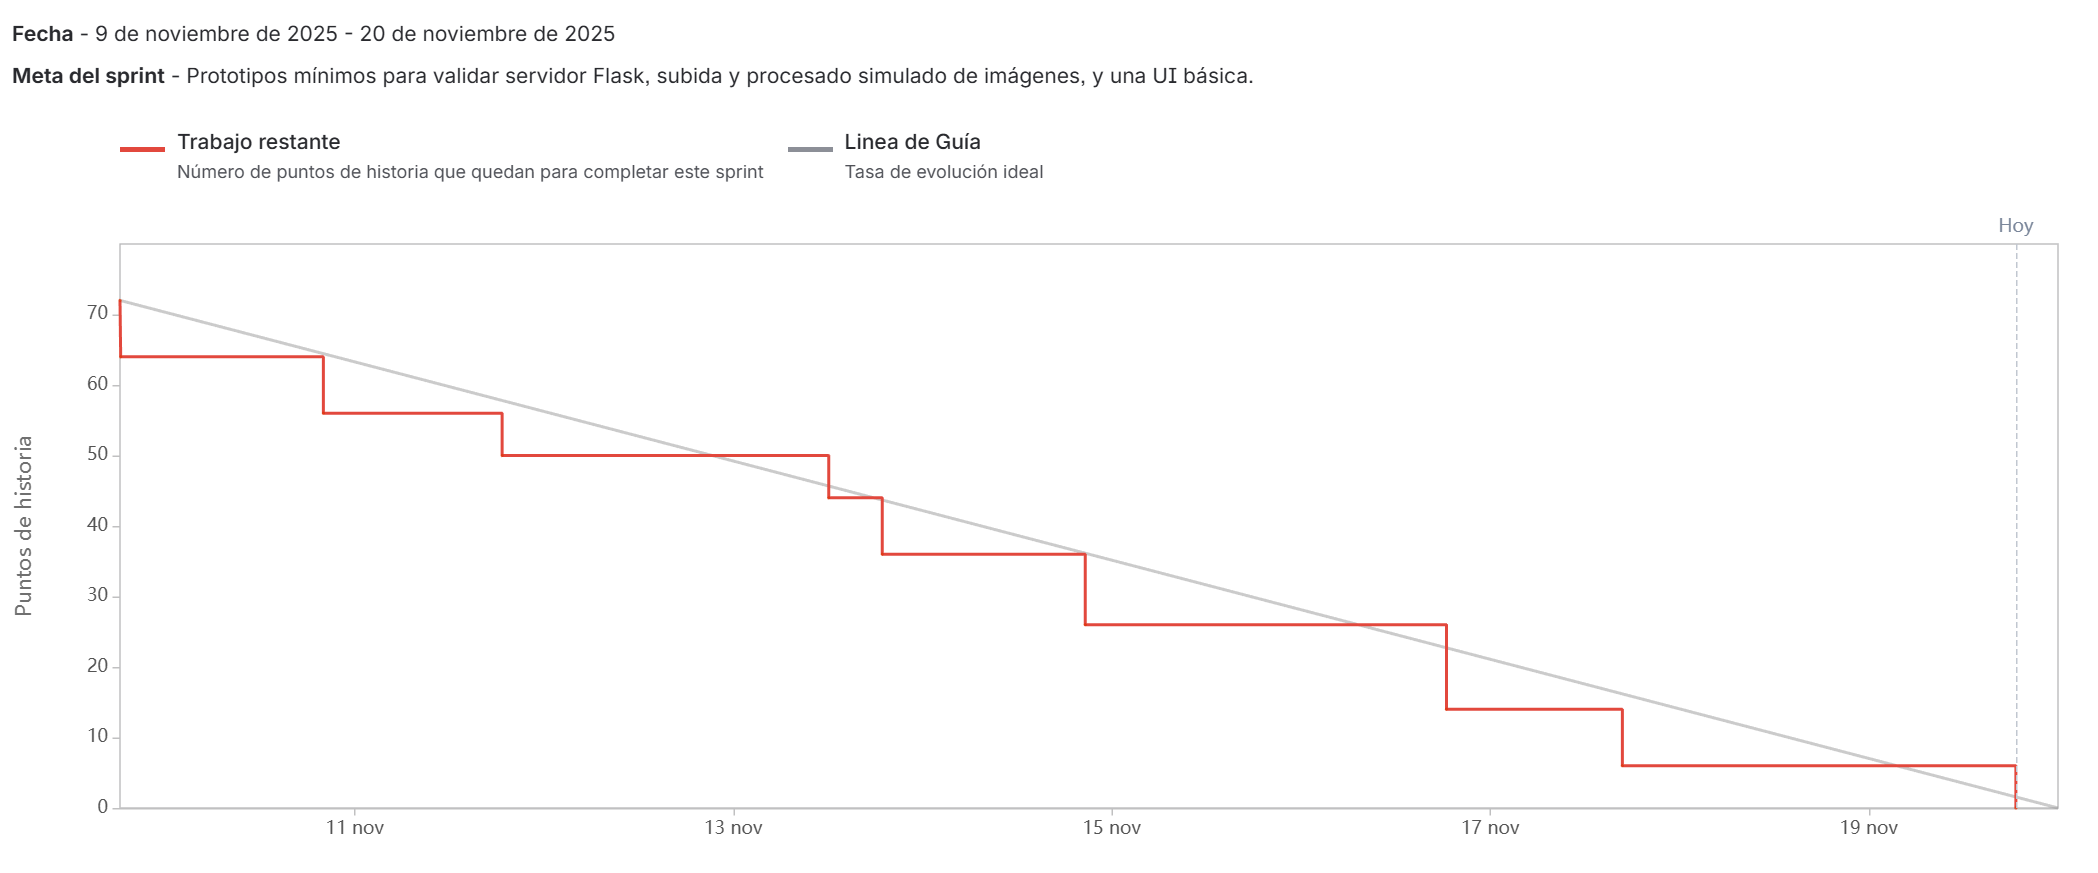
\includegraphics[width=0.95\textwidth]{img/sprint2.png}
	\caption{Informe de trabajo completado Sprint 2}
	\label{fig:sprint2}
\end{figure}

\subsubsection*{Descripción de las tareas del Sprint 2}

A continuación se describen brevemente las tareas realizadas durante este sprint:

\begin{itemize}
	\item \textbf{Definir alcance del sprint y crear historias.}  
	Se concretaron los objetivos del sprint y se desglosaron en historias de usuario. 
	
	\item \textbf{Elegir framework servidor.}  
	Tras evaluar distintas opciones, se seleccionó \textbf{Flask} como framework principal por su ligereza, modularidad y facilidad para integrar endpoints REST orientados al procesado de imágenes.
	
	\item \textbf{Elección librería para simulación de detecciones.}  
	Para poder validar el flujo completo antes de integrar YOLO o MediaPipe reales, se creó una librería propia que genera detecciones simuladas (clases, cajas y confianza).
	
	\item \textbf{Configurar entorno de desarrollo y estructura base.}  
	Se construyó una arquitectura inicial organizada en módulos y se configuró un servidor Flask estable listo para ampliaciones.
	
	\item \textbf{Probar funcionamiento del servidor.}  
	Se verificó la ejecución del backend, comprobando rutas, carga de configuraciones, manejo de errores y logs. Esta fase permitió asegurar que el servidor respondía correctamente antes de construir los endpoints principales.
	
	\item \textbf{Desarrollar endpoint para subir imágenes.}  
	Se creó un endpoint capaz de recibir imágenes vía POST, almacenarlas temporalmente y devolver su ruta accesible desde la interfaz.
	
	\item \textbf{Desarrollar endpoint para detección.}  
	Se implementó un endpoint \texttt{/detect} que recibe la imagen subida y devuelve detecciones generadas mediante la librería simulada y posteriormente los endpoint para el procesado de imágenes con yolo y mediapipe aplicando patrón factory.
	
	\item \textbf{Crear interfaz mínima de aplicación.}  
	Se desarrolló una pequeña UI con HTML y JavaScript para permitir al usuario subir imágenes, elegir un modelo disponible y visualizar el resultado generado.
	
	\item \textbf{Validación final y documentación del sprint.}  
	Se revisaron todas las historias completadas, se generaron capturas de evidencia y se documentó el sprint.
\end{itemize}


\subsection*{Visión general del Sprint 3}
\begin{itemize}
	\item \textbf{Fechas:} 14/02 – 19/02
	\item \textbf{Objetivo del sprint:} \emph{Definir un borrador de los requisitos funcionales, requisitos no funcionales y casos de uso del proyecto.}
	\item \textbf{Criterio de aceptación global:} tener suficientes requisitos y casos de uso para cubrir el funcionamiento total de la aplicación.
\end{itemize}

Como se observa en la Tabla~\ref{tabla:sprint3} y la Figura~\ref{fig:sprint3}, este sprint se centra en la definición de requisitos y casos de uso.

\begin{table}[h!]
	\centering
	\begin{tabular}{@{}ll@{}}
		\toprule
		\textbf{Tarea} & \textbf{Pts} \\
		\midrule
		Definición alcance sprint & 2 \\
		Plantear alcance de requisitos y casos de uso & 6 \\
		Definir requisitos funcionales & 8 \\
		Definir requisitos no funcionales & 8 \\
		Definir casos de uso & 16 \\
		\midrule
		\bottomrule
	\end{tabular}
	\caption{Sprint 3 – Resumen}
	\label{tabla:sprint3}
\end{table}

\begin{figure}[h!]
	\centering
	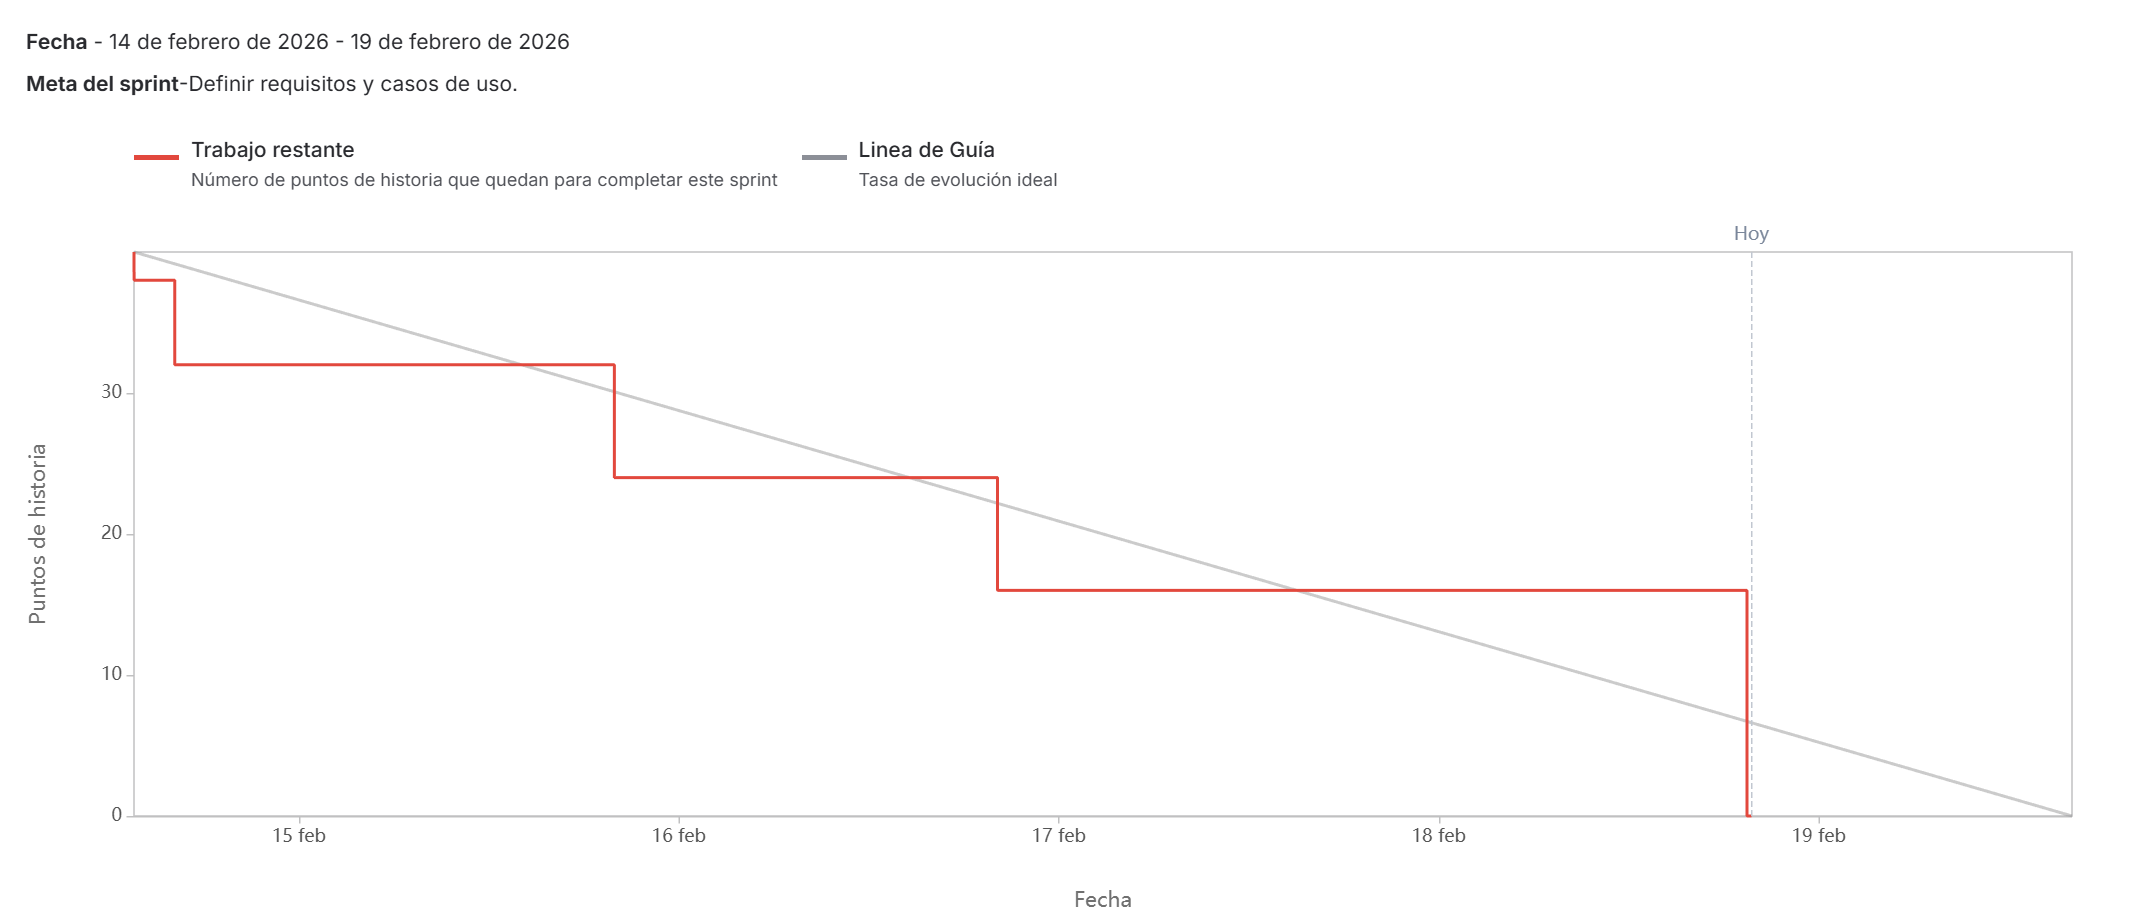
\includegraphics[width=0.95\textwidth]{img/sprint3.png}
	\caption{Informe de trabajo completado Sprint 3}
	\label{fig:sprint3}
\end{figure}

\subsubsection*{Descripción de las tareas del Sprint 3}

Nada importante a destacar en este sprint.

\subsection*{Visión general del Sprint 4}
\begin{itemize}
	\item \textbf{Fechas:} 19/02 – 25/02
	\item \textbf{Objetivo del sprint:} \emph{Completar la documentación del MVP (RF/RNF/CU) y diseñar el modelo E-R de la aplicación (entidades, atributos, relaciones, normalización y reglas).}
	\item \textbf{Criterio de aceptación global:} disponer de la especificación de requisitos del MVP documentada y un modelo E-R completo y coherente (incluyendo normalización, integridad y restricciones de negocio).
\end{itemize}

Tal y como se muestra en la Tabla~\ref{tabla:sprint4} y la Figura~\ref{fig:sprint4}, este sprint se enfoca en el diseño del modelo de datos y la documentación del MVP.

\begin{table}[h!]
	\centering
	\begin{tabular}{@{}ll@{}}
		\toprule
		\textbf{Tarea} & \textbf{Pts} \\
		\midrule
		Corregir y subir documento ``RF\_RNF\_CU\_aplicación\_completa'' & 2 \\
		Documentar los RF/RNF/CU para el producto mínimo viable & 6 \\
		Modelo E-R (identificación de entidades y alcance) & 8 \\
		Modelo E-R (atributos y claves) & 8 \\
		Modelo E-R (relaciones y cardinalidades) & 8 \\
		Modelo E-R (normalización, reglas de integridad y restricciones de negocio) & 8 \\
		\midrule
		\bottomrule
	\end{tabular}
	\caption{Sprint 4 – Resumen}
	\label{tabla:sprint4}
\end{table}

\begin{figure}[h!]
	\centering
	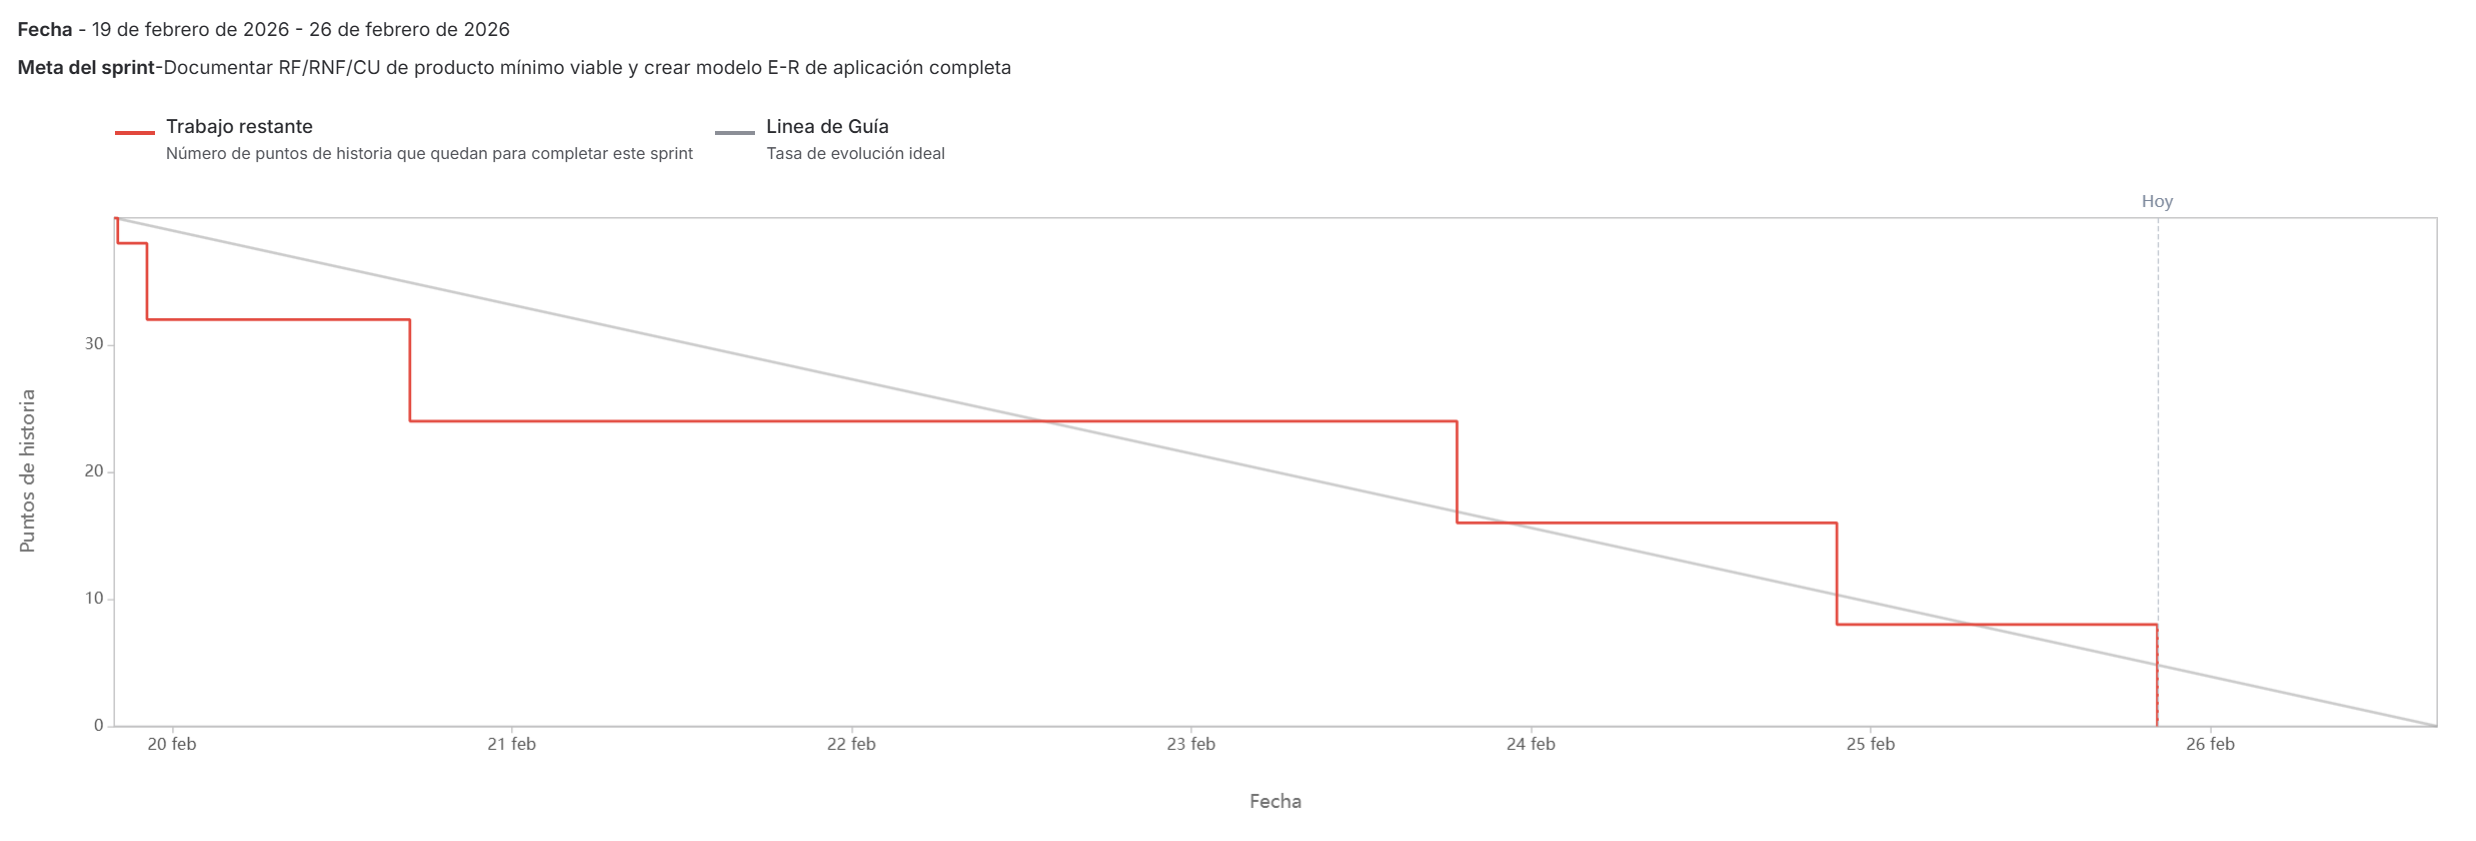
\includegraphics[width=0.95\textwidth]{img/sprint4.png}
	\caption{Informe de trabajo completado Sprint 4}
	\label{fig:sprint4}
\end{figure}

\subsubsection*{Descripción de las tareas del Sprint 4}

A continuación se describen brevemente las tareas realizadas durante este sprint:

\begin{itemize}
	\item \textbf{Corregir y subir documento ``RF\_RNF\_CU\_aplicación\_completa''.}
	Se revisó el documento general de requisitos y casos de uso de la aplicación completa, corrigiendo inconsistencias de redacción y estructura.
	
	\item \textbf{Documentar los RF/RNF/CU para el producto mínimo viable.}
	Se seleccionaron y redactaron los requisitos funcionales y no funcionales junto con los casos de uso estrictamente necesarios para el MVP, priorizando el flujo básico de acceso, selección de IA, envío de imagen y obtención de resultados.
	
	\item \textbf{Modelo E-R (identificación de entidades y alcance).}
	Se identificaron las entidades completas de la aplicación y se delimitó el alcance del modelo para cubrir tanto el MVP como la aplicación completa.
	
	\item \textbf{Modelo E-R (atributos y claves).}
	Se definieron los atributos relevantes de cada entidad y sus claves, estableciendo claves primarias, restricciones de unicidad y una estructura consistente para su posterior representación en el diagrama.
	
	\item \textbf{Modelo E-R (relaciones y cardinalidades).}
	Se diseñó el diagrama E-R utilizando las entidades con sus atributos creados previamente junto definiendo relaciones y cardinalidades que unirían estas.
	
	\item \textbf{Modelo E-R (normalización, reglas de integridad y restricciones de negocio).}
	Se verificó el modelo respecto a formas normales (hasta 3FN) y se definieron reglas de integridad (entidad, referencial y coherencia semántica), además de restricciones de negocio (dominios de estado, coherencia temporal, unicidades y reglas específicas como renovaciones y consistencia IA--modo).
\end{itemize}

\subsection*{Visión general del Sprint 5}
\begin{itemize}
	\item \textbf{Fechas:} 03/03 – 05/03
	\item \textbf{Objetivo del sprint:} \emph{Retroalimentación de diagramas E-R y Relacional.}
	\item \textbf{Criterio de aceptación global:} Tener correcciones hechas sobre los modelos E-R y Relacional de acuerdo a lo comentado en el Sprint Review.
\end{itemize}

Como se refleja en la Tabla~\ref{tabla:sprint5} y la Figura~\ref{fig:sprint5}, este sprint se centra en la mejora de los modelos E-R y relacional.

\begin{table}[h!]
	\centering
	\begin{tabular}{@{}ll@{}}
		\toprule
		\textbf{Tarea} & \textbf{Pts} \\
		\midrule
		Modificar modelo relacional & 8 \\
		Modelo E-R  & 8 \\
		Repasar si E-R y relacional son válidos para casos de uso & 8 \\ \\
		\midrule
		\bottomrule
	\end{tabular}
	\caption{Sprint 5 – Resumen}
	\label{tabla:sprint5}
\end{table}

\begin{figure}[h!]
	\centering
	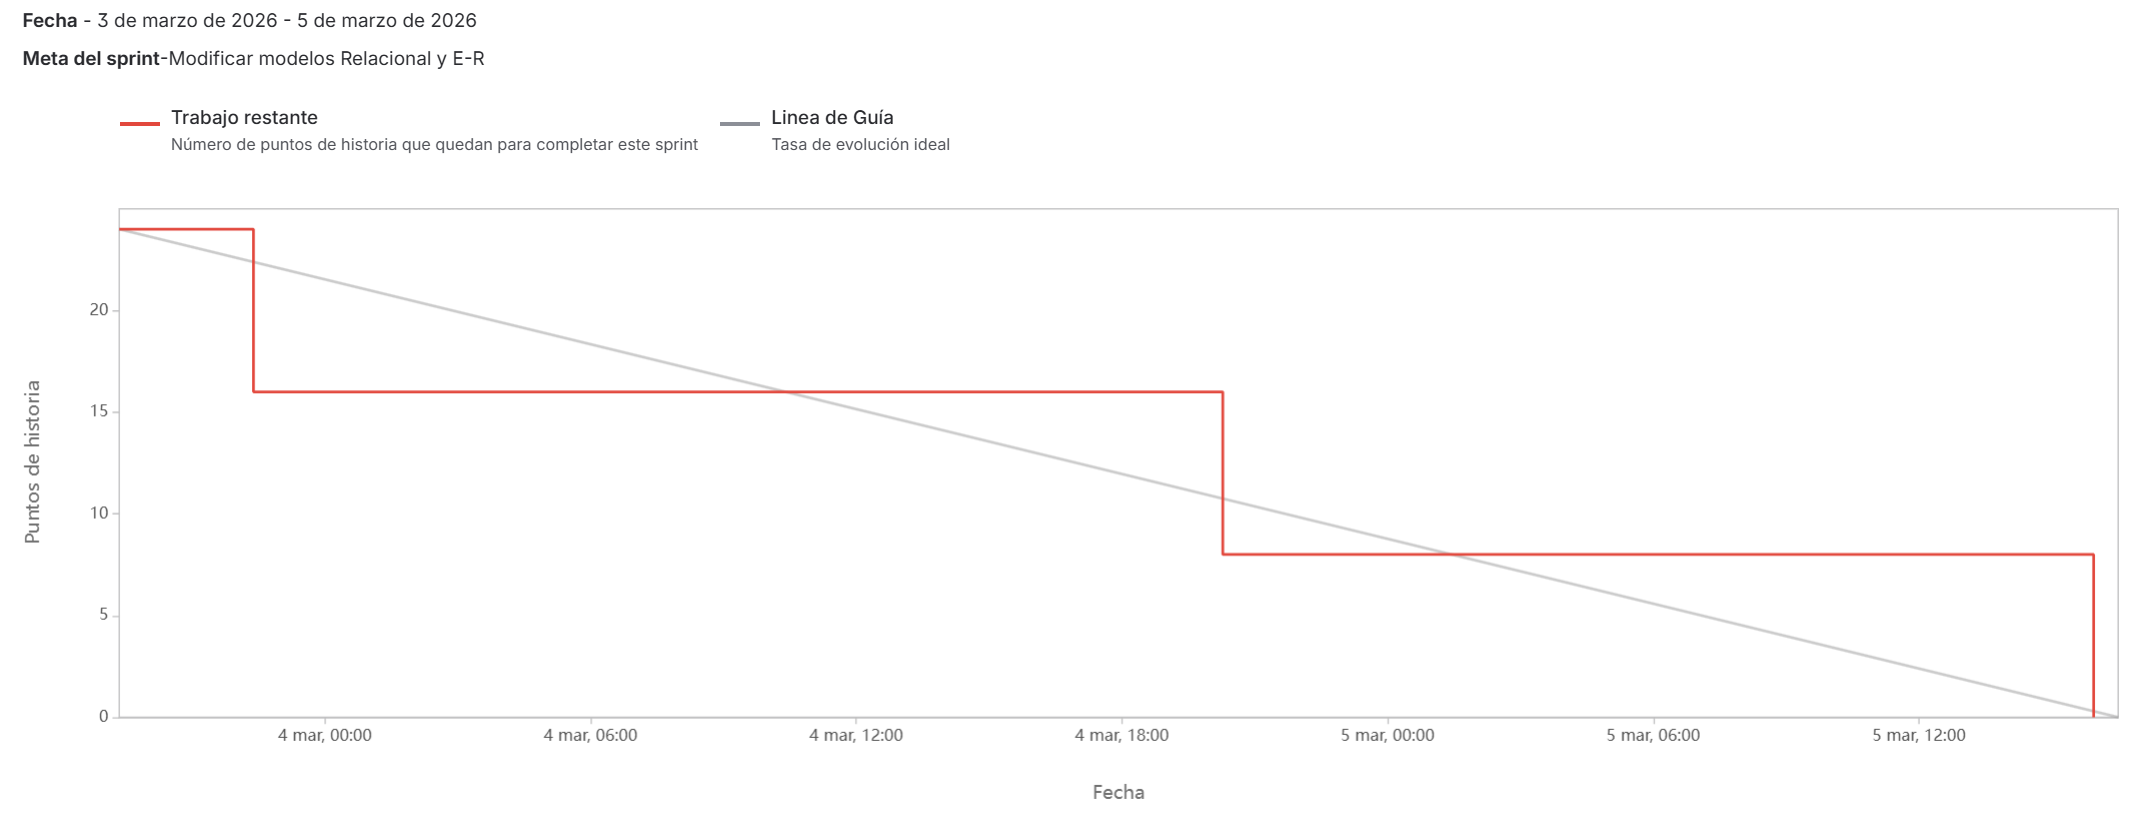
\includegraphics[width=0.95\textwidth]{img/sprint5.png}
	\caption{Informe de trabajo completado Sprint 5}
	\label{fig:sprint5}
\end{figure}

\subsubsection*{Descripción de las tareas del Sprint 5}

A continuación se describen brevemente las tareas realizadas durante este sprint:

\begin{itemize}
	\item \textbf{Modificar modelo relacional.}
	Hacer modificaciones en el modelo relacional para poder estar totalmente normalizado y tener una mejor estructura en cuanto a crecimiento de aplicación.
	
	\item \textbf{Modelo E-R.}
	Realizar el modelo Entidad Relación con la retrospectiva del Sprint Review.
	
	\item \textbf{Repasar si E-R y relacional son válidos para casos de uso.}
	Verificar si con ambos diagramas se podrían llegar a realizar correctamente todos los casos de usos planteados en anteriores sprints.
	
\end{itemize}


\subsection*{Visión general del Sprint 6}
\begin{itemize}
	\item \textbf{Fechas:} 07/03 – 12/03
	\item \textbf{Objetivo del sprint:} \emph{Definir y ajustar el modelo de configuración y ejecución de pipelines.}
	\item \textbf{Criterio de aceptación global:} Tener definidos los criterios de configuración, creación de pipelines y ejecuciones, y reflejarlo en el modelo de datos.
\end{itemize}

Tal y como se muestra en la Tabla~\ref{tabla:sprint6} y la Figura~\ref{fig:sprint6}, este sprint introduce el modelo de pipelines y su configuración.

\begin{table}[h!]
	\centering
	\begin{tabular}{@{}ll@{}}
		\toprule
		\textbf{Tarea} & \textbf{Pts} \\
		\midrule
		Modificación E-R& 4 \\
		Plantear si habrá configuración elegible por el usuario o no & 6 \\
		Plantear si los pipelines los crea el administrador o usuarios & 2 \\
		Plantear si se pueden repetir ejecuciones & 2 \\
		Actualizar modelo respecto a los planteamientos tomados & 10 \\
		Revisar si los requisitos y casos de uso cuadran con respecto a los planteamientos & 8 \\
		\midrule
		\bottomrule
	\end{tabular}
	\caption{Sprint 6 – Resumen}
	\label{tabla:sprint6}
\end{table}

\begin{figure}[h!]
	\centering
	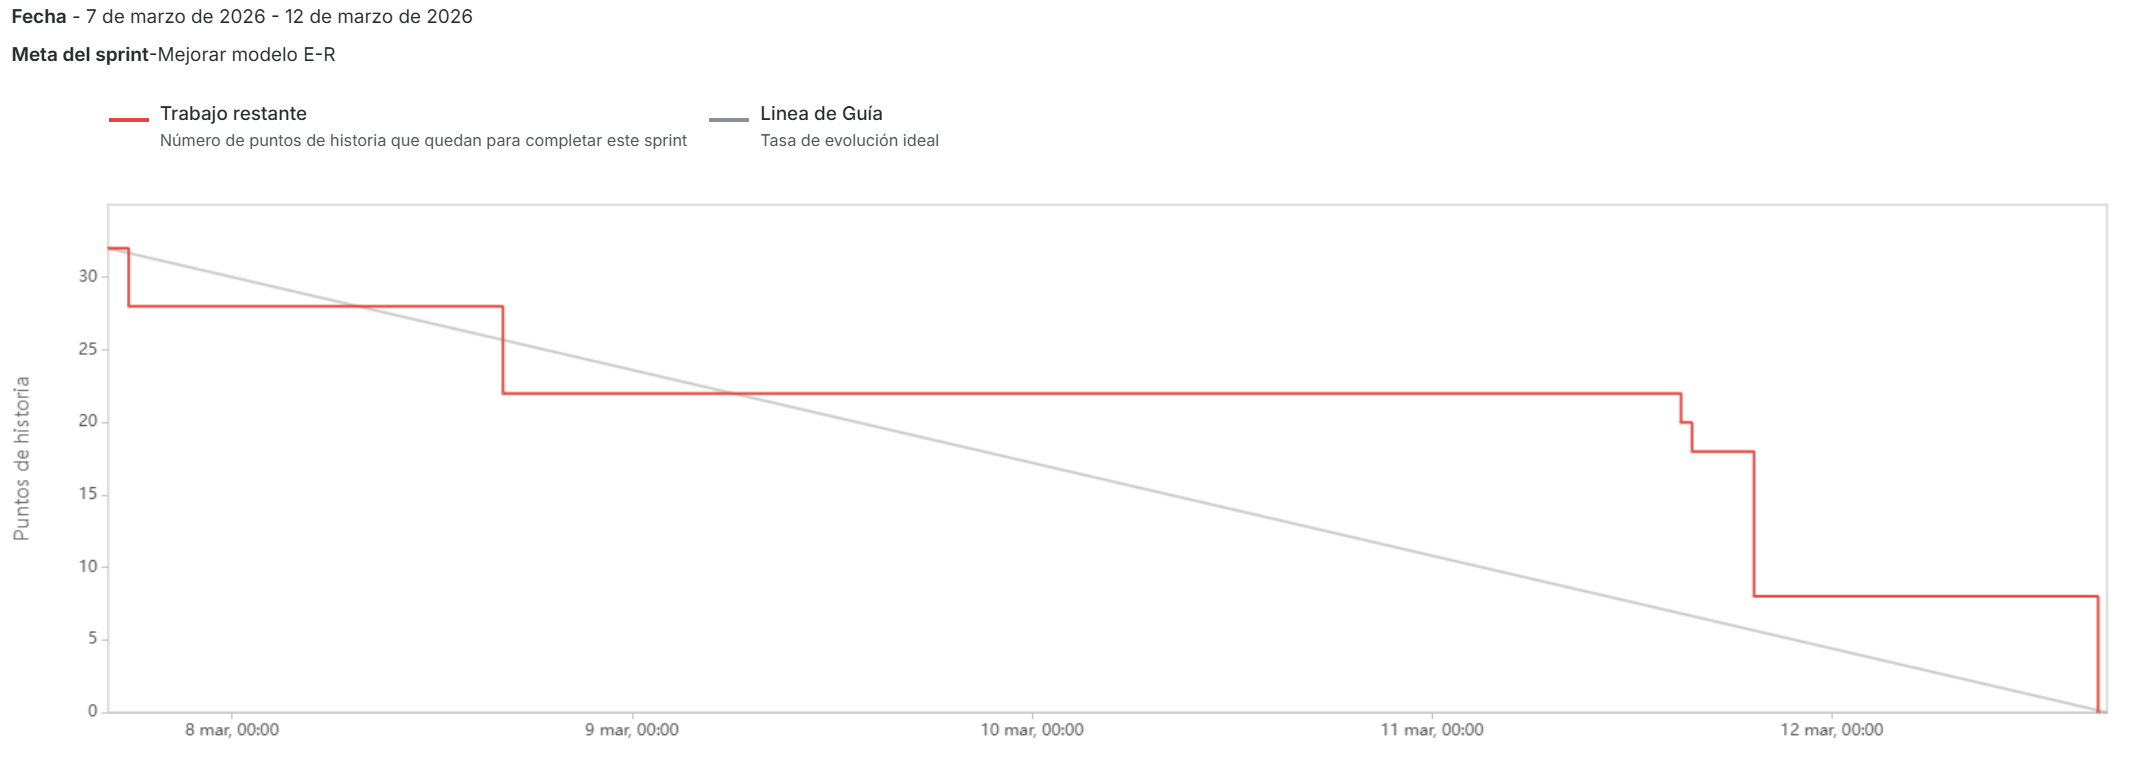
\includegraphics[width=0.95\textwidth]{img/sprint6.png}
	\caption{Informe de trabajo completado Sprint 6}
	\label{fig:sprint6}
\end{figure}

\subsubsection*{Descripción de las tareas del Sprint 6}

A continuación se describen brevemente las tareas realizadas durante este sprint:

\begin{itemize}
	
	\item \textbf{Modificación E-R.}
	Ajustar el diagrama E-R según los nuevos planteamientos.
	
	\item \textbf{Plantear si habrá configuración elegible por el usuario o no.}
	Analizar si los usuarios pueden modificar configuraciones.
	
	\item \textbf{Plantear si los pipelines los crea el administrador o usuarios.}
	Determinar si los pipelines los crea el administrador o los usuarios.
	
	\item \textbf{Plantear si se pueden repetir ejecuciones.}
	Estudiar si las ejecuciones pueden repetirse.
	
	\item \textbf{Actualizar modelo respecto a los planteamientos tomados.}
	Reflejar las decisiones tomadas en el modelo de datos.
	
	\item \textbf{Revisar si los requisitos y casos de uso cuadran con respecto a los planteamientos.}
	Comprobar coherencia entre requisitos, casos de uso y modelo.
	
\end{itemize}


\subsection*{Visión general del Sprint 7}
\begin{itemize}
	\item \textbf{Fechas:} 16/03 – 19/03
	\item \textbf{Objetivo del sprint:} \emph{Preparar el entorno de desarrollo definitivo en Debian e iniciar la implementación real de la base de datos del sistema.}
	\item \textbf{Criterio de aceptación global:} Disponer de un entorno funcional en Debian con MariaDB operativo y haber comenzado la implementación física de la base de datos a partir de los diagramas diseñados.
\end{itemize}

Tal y como se muestra en la Tabla~\ref{tabla:sprint7} y la Figura~\ref{fig:sprint7}, este sprint se centra en la transición desde un entorno de desarrollo inicial hacia un entorno más realista y alineado con el despliegue final, así como en el inicio de la materialización del modelo de datos definido en fases anteriores.

\begin{table}[h!]
	\centering
	\begin{tabular}{@{}ll@{}}
		\toprule
		\textbf{Tarea} & \textbf{Pts} \\
		\midrule
		Crear Debian en dual boot con Windows & 8 \\
		Preparar Debian con configuración mínima & 4 \\
		Instalar MariaDB & 4 \\
		Pruebas MariaDB & 8 \\
		Empezar base de datos TFG & 8 \\
		\midrule
		\bottomrule
	\end{tabular}
	\caption{Sprint 7 – Resumen}
	\label{tabla:sprint7}
\end{table}

\begin{figure}[h!]
	\centering
	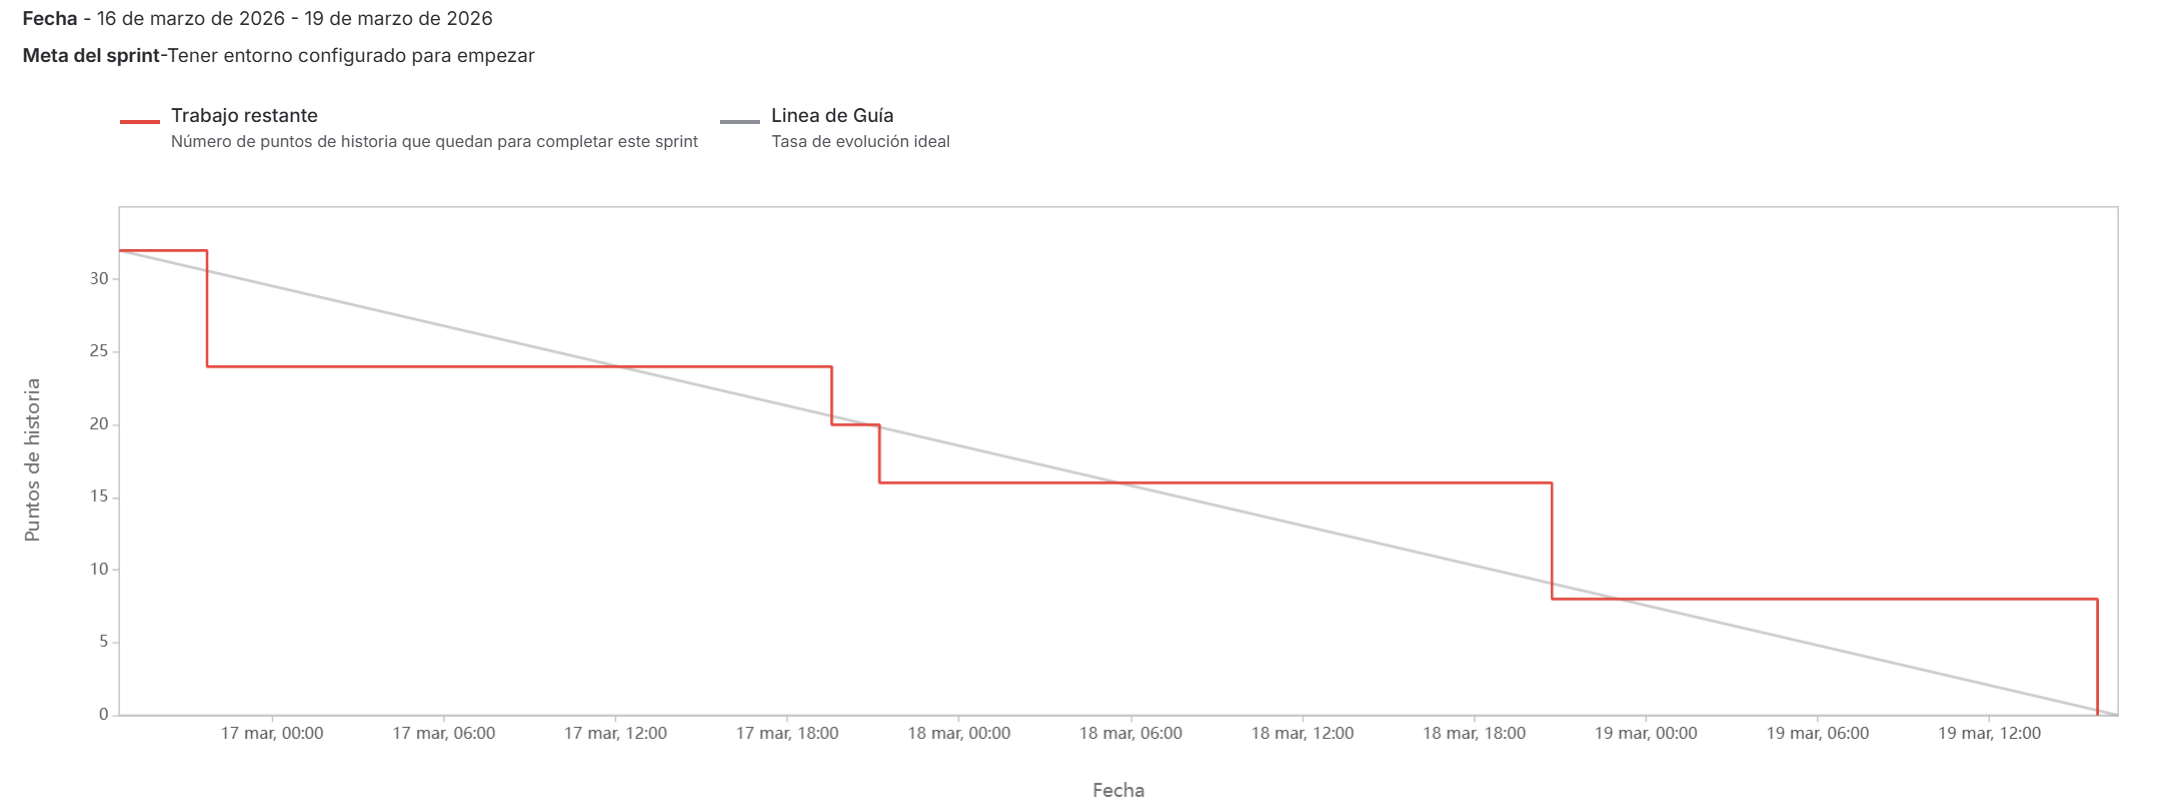
\includegraphics[width=0.95\textwidth]{img/sprint7.png}
	\caption{Informe de trabajo completado Sprint 7}
	\label{fig:sprint7}
\end{figure}

\subsubsection*{Descripción de las tareas del Sprint 7}

A continuación se describen brevemente las tareas realizadas durante este sprint:

\begin{itemize}
	
	\item \textbf{Crear Debian en dual boot con Windows}  
	Se realizó la instalación de Debian en configuración de arranque dual con Windows con el objetivo de disponer de un entorno de desarrollo más estable, controlado y alineado con el entorno de despliegue final en servidores Linux.
	
	\item \textbf{Preparar Debian con configuración mínima}  
	Configuración inicial del sistema con las herramientas básicas necesarias para el desarrollo.
	
	\item \textbf{Instalar MariaDB}  
	Instalación del sistema gestor de bases de datos que será utilizado en el proyecto.
	
	\item \textbf{Pruebas MariaDB}  
	Verificación del correcto funcionamiento de MariaDB mediante pruebas básicas de conexión y ejecución de consultas.
	
	\item \textbf{Empezar base de datos TFG}  
	Inicio de la implementación física de la base de datos, trasladando los diagramas entidad-relación y el modelo relacional definidos previamente a tablas reales en MariaDB.
	
\end{itemize}


\subsection*{Visión general del Sprint 8}
\begin{itemize}
	\item \textbf{Fechas:} 20/03 – 26/03
	\item \textbf{Objetivo del sprint:} \emph{Ajustar el diseño del modelo de datos e implementar completamente la base de datos del sistema.}
	\item \textbf{Criterio de aceptación global:} Disponer de una base de datos completamente implementada en MariaDB y coherente con el modelo relacional actualizado.
	\item \textbf{Explicación sprint retrasado:} Sufrí una baja médica.
\end{itemize}

Tal y como se muestra en la Tabla~\ref{tabla:sprint8} y la Figura~\ref{fig:sprint8}, este sprint se centra en consolidar el diseño de datos mediante su ajuste durante la implementación real, así como en completar la construcción de la base de datos del sistema.

\begin{table}[h!]
	\centering
	\begin{tabular}{@{}ll@{}}
		\toprule
		\textbf{Tarea} & \textbf{Pts} \\
		\midrule
		Actualizar modelo relacional & 4 \\
		Implementar base de datos & 12 \\
		Documentar base de datos & 10 \\
		Documentar aspectos relevantes memoria & 10 \\
		Añadir referencias a imágenes y tablas en anexos & 4 \\
		\midrule
		\bottomrule
	\end{tabular}
	\caption{Sprint 8 – Resumen}
	\label{tabla:sprint8}
\end{table}

\begin{figure}[h!]
	\centering
	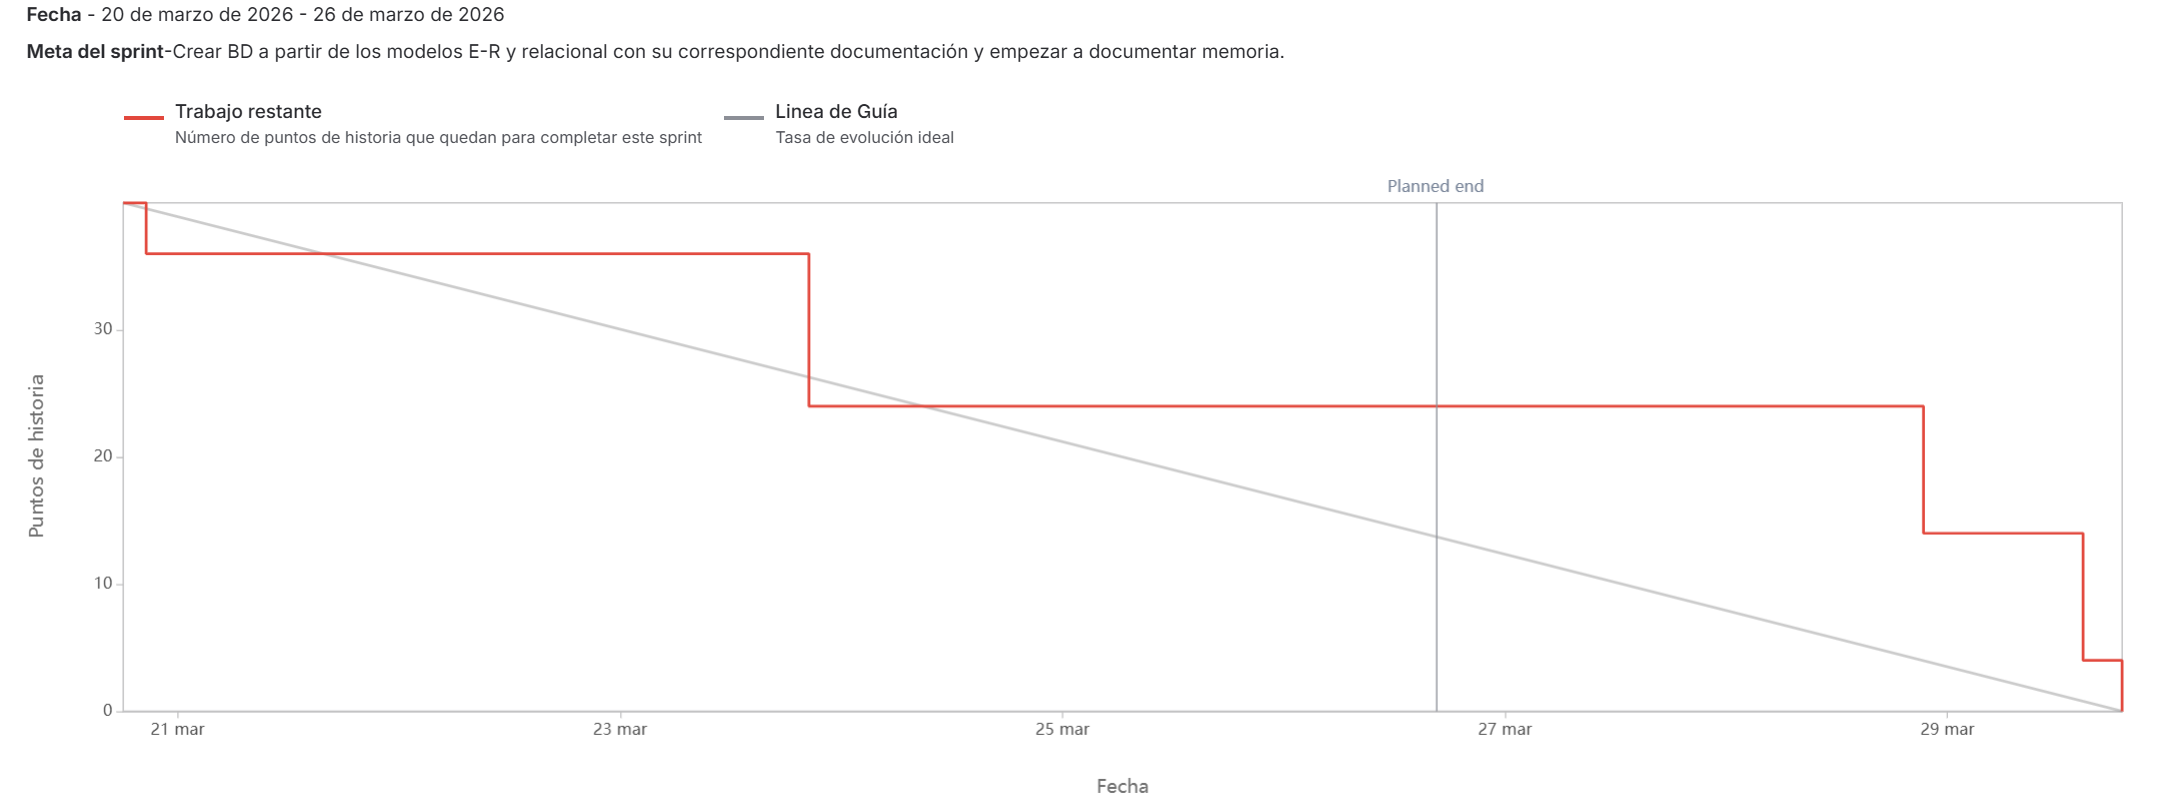
\includegraphics[width=0.95\textwidth]{img/sprint8.png}
	\caption{Informe de trabajo completado Sprint 8}
	\label{fig:sprint8}
\end{figure}

\subsubsection*{Descripción de las tareas del Sprint 8}

A continuación se describen brevemente las tareas realizadas durante este sprint:

\begin{itemize}
	
	\item \textbf{Actualizar modelo relacional}  
	Se realizaron ajustes en el modelo relacional a partir de los cambios detectados durante la implementación de la base de datos.
	
	\item \textbf{Implementar base de datos}  
	Construcción completa de la base de datos en MariaDB a partir del modelo relacional definido.
	
	\item \textbf{Documentar base de datos}  
	Elaboración de la documentación asociada al diseño e implementación de la base de datos.
	
	\item \textbf{Documentar aspectos relevantes memoria}  
	Redacción de los aspectos clave del desarrollo para su inclusión en la memoria del TFG.
	
	\item \textbf{Añadir referencias a imágenes y tablas en anexos}  
	Incorporación de referencias cruzadas a figuras y tablas dentro de los anexos.
	
\end{itemize}

\subsection*{Visión general del Sprint 9}
\begin{itemize}
	\item \textbf{Fechas:} 06/04 – 09/04
	\item \textbf{Objetivo del sprint:} \emph{Definir la estructura base del sistema bajo el patrón MVC e integrar los primeros componentes funcionales del backend y la interfaz.}
	\item \textbf{Criterio de aceptación global:} Disponer de una arquitectura MVC funcional con modelos de IA operativos, autenticación básica de usuarios y una interfaz mínima de interacción.
\end{itemize}

Tal y como se muestra en la Tabla~\ref{tabla:sprint9} y la Figura~\ref{fig:sprint9}, este sprint marca el inicio de la construcción de la aplicación como sistema estructurado, pasando de componentes aislados a una arquitectura organizada basada en el patrón Modelo-Vista-Controlador.

\begin{table}[h!]
	\centering
	\begin{tabular}{@{}ll@{}}
		\toprule
		\textbf{Tarea} & \textbf{Pts} \\
		\midrule
		Crear primera estructura modelo vista controlador & 12 \\
		Poner en funcionamiento los modelos en el modelo & 8 \\
		Poner en funcionamiento usuarios en el modelo & 6 \\
		Crear interfaz mínima & 6 \\
		\midrule
		\bottomrule
	\end{tabular}
	\caption{Sprint 9 – Resumen}
	\label{tabla:sprint9}
\end{table}

\begin{figure}[h!]
	\centering
	\includegraphics[width=0.95\textwidth]{img/sprint9.png}
	\caption{Informe de trabajo completado Sprint 9}
	\label{fig:sprint9}
\end{figure}

\subsubsection*{Descripción de las tareas del Sprint 9}

A continuación se describen brevemente las tareas realizadas durante este sprint:

\begin{itemize}
	
	\item \textbf{Crear primera estructura modelo vista controlador}  
	Definición de la estructura base del sistema siguiendo el patrón MVC, estableciendo la organización inicial de carpetas, módulos y responsabilidades.
	
	\item \textbf{Poner en funcionamiento los modelos en el modelo}  
	Integración de los modelos de IA dentro de la arquitectura MVC para su ejecución desde la lógica de negocio.
	
	\item \textbf{Poner en funcionamiento usuarios en el modelo}  
	Implementación de un sistema básico de autenticación que permite el inicio de sesión de usuarios.
	
	\item \textbf{Crear interfaz mínima}  
	Desarrollo de una interfaz sencilla que permite visualizar y probar el funcionamiento básico de la aplicación de forma gráfica.
	
\end{itemize}


\subsection*{Visión general del Sprint 10}
\begin{itemize}
	\item \textbf{Fechas:} 13/04 – 16/04
	\item \textbf{Objetivo del sprint:} \emph{Mejorar la calidad de la documentación y avanzar en la implementación del sistema de autenticación en la interfaz.}
	\item \textbf{Criterio de aceptación global:} Disponer de una documentación más refinada y de un sistema de inicio de sesión funcional desde la interfaz gráfica con diferenciación básica de roles.
\end{itemize}

Tal y como se muestra en la Tabla~\ref{tabla:sprint10} y la Figura~\ref{fig:sprint10}, este sprint se centra en mejorar la calidad de la documentación del proyecto y en avanzar hacia una interacción más completa del usuario con la aplicación mediante autenticación desde la interfaz.

\begin{table}[h!]
	\centering
	\begin{tabular}{@{}ll@{}}
		\toprule
		\textbf{Tarea} & \textbf{Pts} \\
		\midrule
		Corregir problemas con documentación & 3 \\
		Mejorar documentación técnicas y herramientas & 5 \\
		Reducir aspectos relevantes de tamaño & 8 \\
		Empezar con inicio sesión de usuarios & 16 \\
		\midrule
		\bottomrule
	\end{tabular}
	\caption{Sprint 10 – Resumen}
	\label{tabla:sprint10}
\end{table}

\begin{figure}[h!]
	\centering
	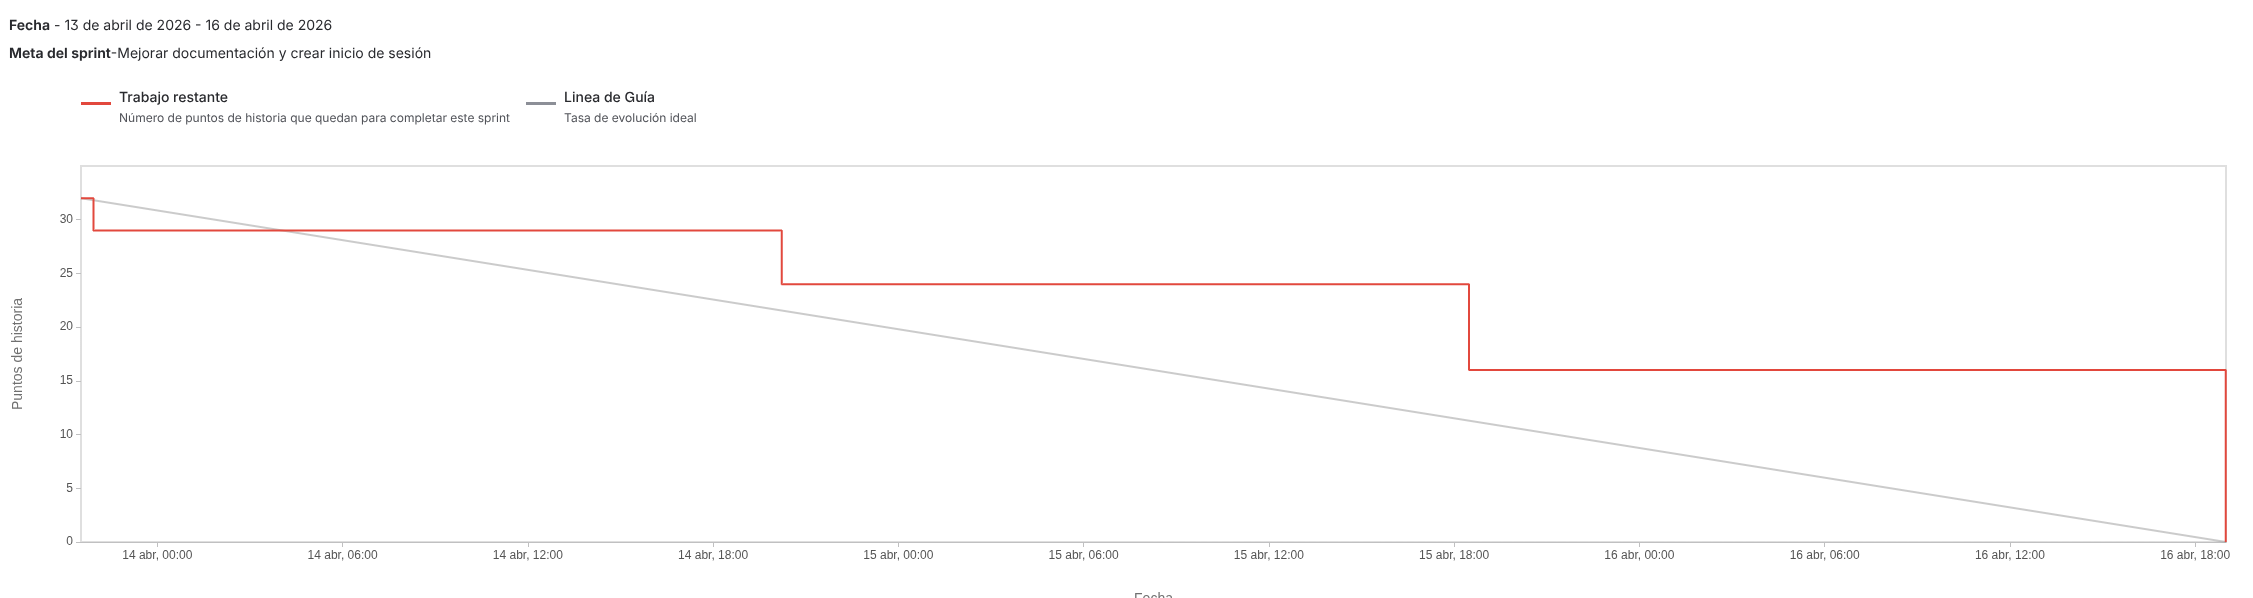
\includegraphics[width=0.95\textwidth]{img/sprint10.png}
	\caption{Informe de trabajo completado Sprint 10}
	\label{fig:sprint10}
\end{figure}

\subsubsection*{Descripción de las tareas del Sprint 10}

A continuación se describen brevemente las tareas realizadas durante este sprint:

\begin{itemize}
	
	\item \textbf{Corregir problemas con documentación}  
	Corrección de errores de formato y estructura detectados en la documentación del proyecto.
	
	\item \textbf{Mejorar documentación técnicas y herramientas}  
	Refinamiento de la sección de técnicas y herramientas utilizadas en el TFG.
	
	\item \textbf{Reducir aspectos relevantes de tamaño}  
	Ajuste del contenido de la memoria para mejorar su claridad y adecuación al formato requerido.
	
	\item \textbf{Empezar con inicio sesión de usuarios}  
	Implementación del inicio de sesión desde la interfaz gráfica, incluyendo la separación de vistas entre usuarios normales y administradores.
	
\end{itemize}




\section{Estudio de viabilidad}

\subsection{Viabilidad económica}

\subsection{Viabilidad legal}


